\section{Orbits in an axisymmetric potential}
Considering an axisymmetric potential used as a simple model for a galaxian disk first proposed by Toomre (1964, ApJ):
\begin{equation}
    U(r) = -(1+r^2)^{-1/2}.
\end{equation}


%%%%%%%%%%%%%%%%%%%%%%%%%%%%%%%%%%%%%%%%%%%%%%%%%%%%%%%%%%%%%%%
%=========================SUBSECTION===========================
%%%%%%%%%%%%%%%%%%%%%%%%%%%%%%%%%%%%%%%%%%%%%%%%%%%%%%%%%%%%%%%
\subsection{}
% (a) Pick some initial conditions and integrate the orbits using your
% orbit integration code. Verify that orbits do not close but precess.
% These are sometimes called rosette orbits because of their shape
% or tube orbits because the have an inner and outer boundary.

\begin{table}[h!]
  \begin{center}
    \caption{Autogenerated table from .csv file.}
    \label{table1}
    \pgfplotstabletypeset[
      multicolumn names, % allows to have multicolumn names
      col sep=comma, % the seperator in our .csv file
      display columns/0/.style={
		column name=$Value 1$, % name of first column
		column type={S},string type},  % use siunitx for formatting
      display columns/1/.style={
		column name=$Value 2$,
		column type={S},string type},
      every head row/.style={
		before row={\toprule}, % have a rule at top
		after row={
			\si{\ampere} & \si{\volt}\\ % the units seperated by &
			\midrule} % rule under units
			},
		every last row/.style={after row=\bottomrule}, % rule at bottom
    ]{CodeAndFigures/ToomreOrbitsData.csv} % filename/path to file
  \end{center}
\end{table}

%%%%%%%%%%%%%%%%%%%%%%%%%%%%%%%%%%%%%%%%%%%%%%%%%%%%%%%%%%%%%%%
%=========================SUBSECTION===========================
%%%%%%%%%%%%%%%%%%%%%%%%%%%%%%%%%%%%%%%%%%%%%%%%%%%%%%%%%%%%%%%
\subsection{}
% (b) Compute the energy and angular momentum of your trial orbits
% (e.g. using the initial conditions). Compute the inner and outer
% radii of the tube (the turning points) using the conserved quantities
% and check these values against your direct orbit integration.

\begin{figure*}
    \centering
    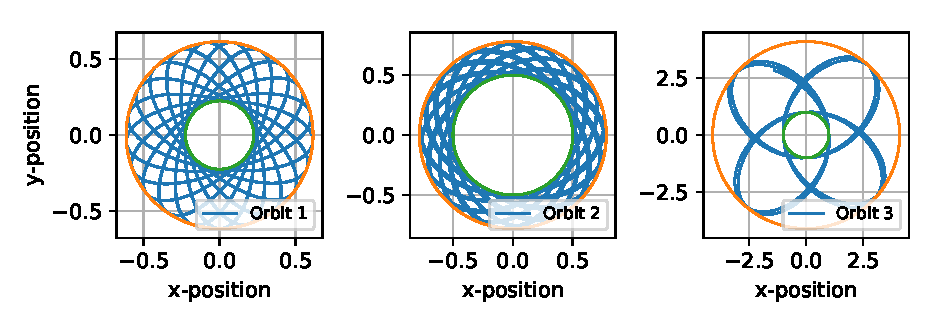
\includegraphics{CodeAndFigures/ToomrePotentialOrbits.pdf}
    \caption{Rosette Orbits using initial conditions of Left: $x=.3$, $y=0$, $v_x=.3$ and $v_y=.4$ Middle: $x=0$, $y=0.5$, $v_x=.6$ and $v_y=0$. Right:$x=1$, $y=0$, $v_x=0$ and $v_y=1$.}
    \label{fig:ToomreOrbits}
\end{figure*}

\begin{figure*}
    \centering
    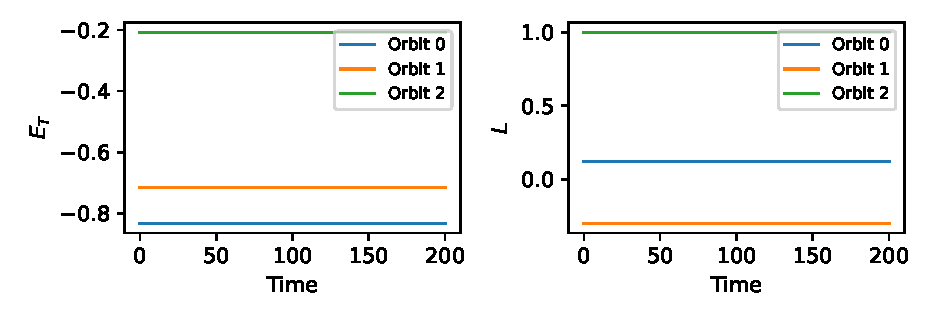
\includegraphics{CodeAndFigures/EnergyMomentumPlot.pdf}
    \caption{Left: Energy and Right: Angular Momentum of the rosette orbits in function with time.}
    \label{fig:ToomreOrbits}
\end{figure*}
